% =============================================================================
% PART B - MODULE 13: CONTRACT MANAGEMENT (UC-13.01 - UC-13.12)
% In Charge: Vo Nhut Tin (CE180619)
% =============================================================================

\newpage
\subsection{Module 13: Contract Management}

The Contract Management module governs the complete contractual lifecycle between Clients and Freelancers on \textbf{Frevia}---from hiring a winning proposal with milestone allocations and pre-signature Stripe escrow holds to bilateral digital signatures, PDF agreement downloads, shared contract attachments, formal cancellation, or contract completion.

% -----------------------------------------------------------------------------
\subsubsection[M13.01 -- Create Contract (UC-13.01)]{M13.01 -- Create Contract \& Hire Freelancer (UC-13.01)}

\begin{itemize}[leftmargin=1.5em,itemsep=2pt]
  \item \textbf{Screen Name \& Route Path:} Create Contract \& Hire Freelancer Drawer -- \texttt{/client/\allowbreak{}jobs/\allowbreak{}[id]/\allowbreak{}proposals}.
  \item \textbf{Target Actor:} Client.
  \item \Needspace{6\baselineskip}\textbf{Before You Begin:} You have an open job posting with at least one submitted proposal (\texttt{SUBMITTED}) and available hiring slots.
\end{itemize}
\begin{figure}[H]\centering
  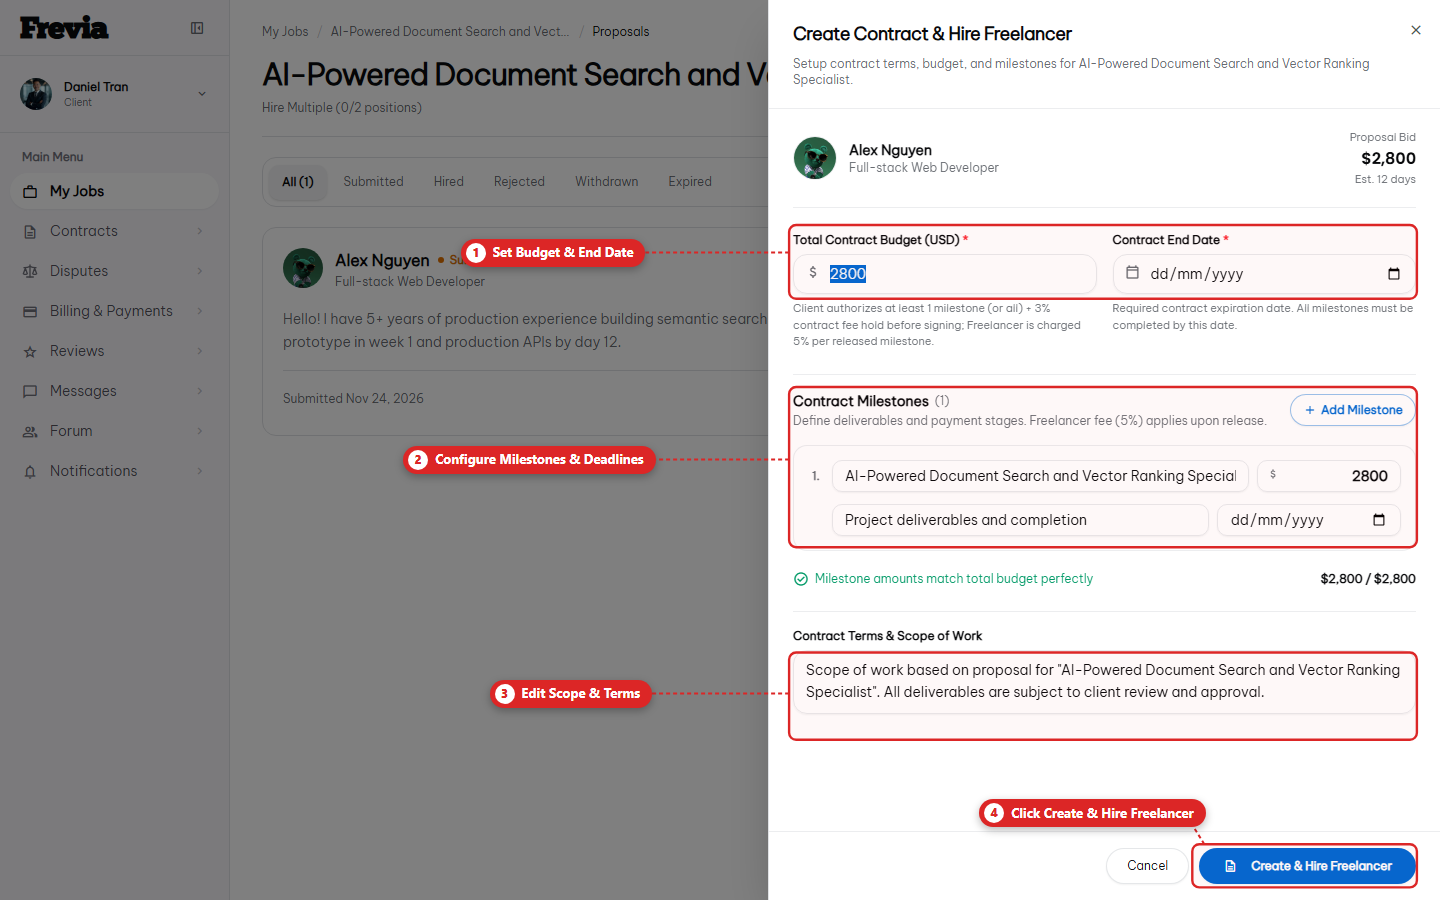
\includegraphics[width=0.90\textwidth]{images/contracts/m13_01_create_contract_guide.png}
  \caption{Create Contract \& Hire Freelancer drawer with milestone builder}
  \label{fig:m13_01_create_contract}
\end{figure}
\Needspace{6\baselineskip}\paragraph{Step-by-Step User Guide:}
\begin{enumerate}[leftmargin=1.8em,itemsep=3pt]
  \item \rbadge{1} \textbf{Set Budget \& End Date:} Review or edit \textit{Total Contract Budget (USD)} and select the required future \textit{Contract End Date}.
  \item \rbadge{2} \textbf{Configure Milestones \& Deadlines:} Verify or split deliverables into scheduled payment milestones via \textbf{+ Add Milestone}, ensuring each milestone due date falls on or before the Contract End Date and sums match the total budget.
  \item \rbadge{3} \textbf{Edit Scope \& Terms:} Customize \textit{Contract Terms \& Scope of Work} governing delivery expectations and acceptance rules.
  \item \rbadge{4} \textbf{Click Create \& Hire Freelancer:} Click \textbf{Create \& Hire Freelancer} to issue the contract (\texttt{AWAITING\_PAYMENT} until the initial Stripe hold is authorized).
\end{enumerate}
\Needspace{6\baselineskip}\paragraph{After You Submit (Result \& Troubleshooting):}
\begin{itemize}[leftmargin=1.5em,itemsep=2pt]
  \item \textbf{What Happens Next:} The contract and its milestone records are created in PostgreSQL, the proposal updates to \texttt{HIRED}, and the Freelancer receives an in-app notification.
  \item \textbf{Troubleshooting \& Common Messages:} Ensure milestone amounts match \textit{Total Contract Budget} (otherwise HTTP 422 \textit{MilestoneAmountMismatch} is returned) and no milestone due date exceeds \textit{Contract End Date}.
\end{itemize}

% -----------------------------------------------------------------------------
\newpage
\subsubsection[M13.02 -- Update Contract (UC-13.02)]{M13.02 -- Update Contract Terms \& Schedule (UC-13.02)}

\begin{itemize}[leftmargin=1.5em,itemsep=2pt]
  \item \textbf{Screen Name \& Route Path:} Edit Contract Agreement Drawer -- \texttt{/client/\allowbreak{}contracts/\allowbreak{}[slug]}.
  \item \textbf{Target Actor:} Client.
  \item \Needspace{6\baselineskip}\textbf{Before You Begin:} Open the contract workspace and click \textbf{Edit Scope \& Terms} while the contract has not yet been signed by both parties.
\end{itemize}
\begin{figure}[H]\centering
  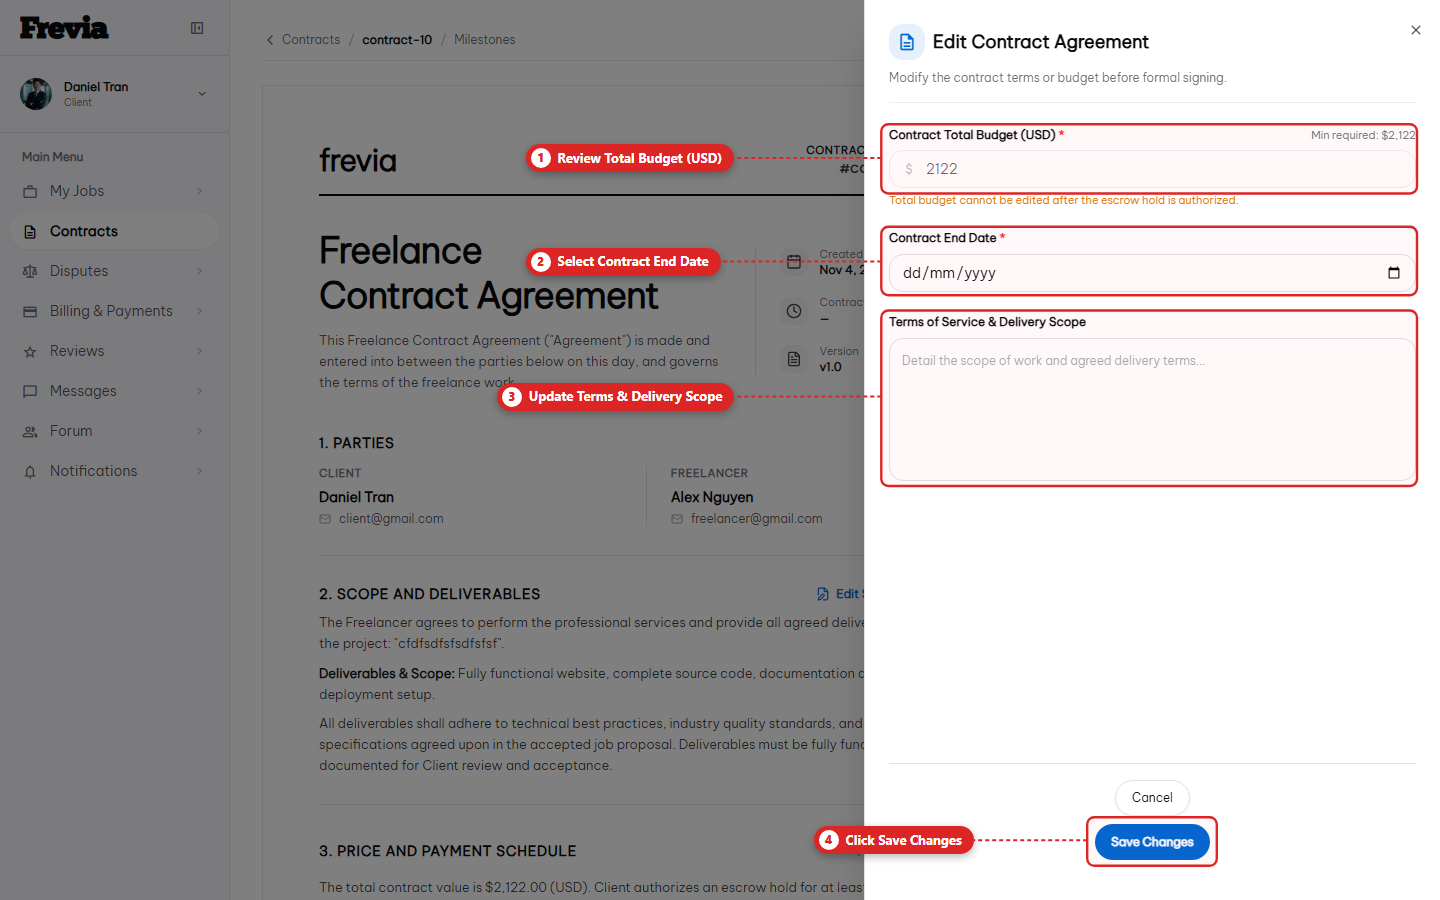
\includegraphics[width=0.90\textwidth]{images/contracts/m13_02_update_contract_guide.png}
  \caption{Edit Contract Agreement drawer for modifying end date and terms}
  \label{fig:m13_02_update_contract}
\end{figure}
\Needspace{6\baselineskip}\paragraph{Step-by-Step User Guide:}
\begin{enumerate}[leftmargin=1.8em,itemsep=3pt]
  \item \rbadge{1} \textbf{Review Total Budget (USD):} Check the contract total budget (locked automatically once the Stripe escrow hold is authorized).
  \item \rbadge{2} \textbf{Select Contract End Date:} Pick a valid future \textit{Contract End Date} covering all planned milestones.
  \item \rbadge{3} \textbf{Update Terms \& Delivery Scope:} Modify the contractual clauses and scope obligations in \textit{Terms of Service \& Delivery Scope}.
  \item \rbadge{4} \textbf{Click Save Changes:} Click the blue \textbf{Save Changes} button to persist updated terms and increment agreement readiness.
\end{enumerate}
\Needspace{6\baselineskip}\paragraph{After You Submit (Result \& Troubleshooting):}
\begin{itemize}[leftmargin=1.5em,itemsep=2pt]
  \item \textbf{What Happens Next:} The contract document updates immediately and notifies the Freelancer of any modified clauses or deadlines.
  \item \textbf{Troubleshooting \& Common Messages:} Budget fields become read-only after escrow authorization; end dates cannot precede existing milestone due dates.
\end{itemize}

% -----------------------------------------------------------------------------
\newpage
\subsubsection{M13.03 -- View Contracts List (UC-13.04)}

\begin{itemize}[leftmargin=1.5em,itemsep=2pt]
  \item \textbf{Screen Name \& Route Path:} My Contracts Dashboard -- \texttt{/client/\allowbreak{}contracts} or \texttt{/freelancer/\allowbreak{}contracts}.
  \item \textbf{Target Actor:} Client, Freelancer.
  \item \Needspace{6\baselineskip}\textbf{Before You Begin:} Signed in with an active Client or Freelancer session.
\end{itemize}
\begin{figure}[H]\centering
  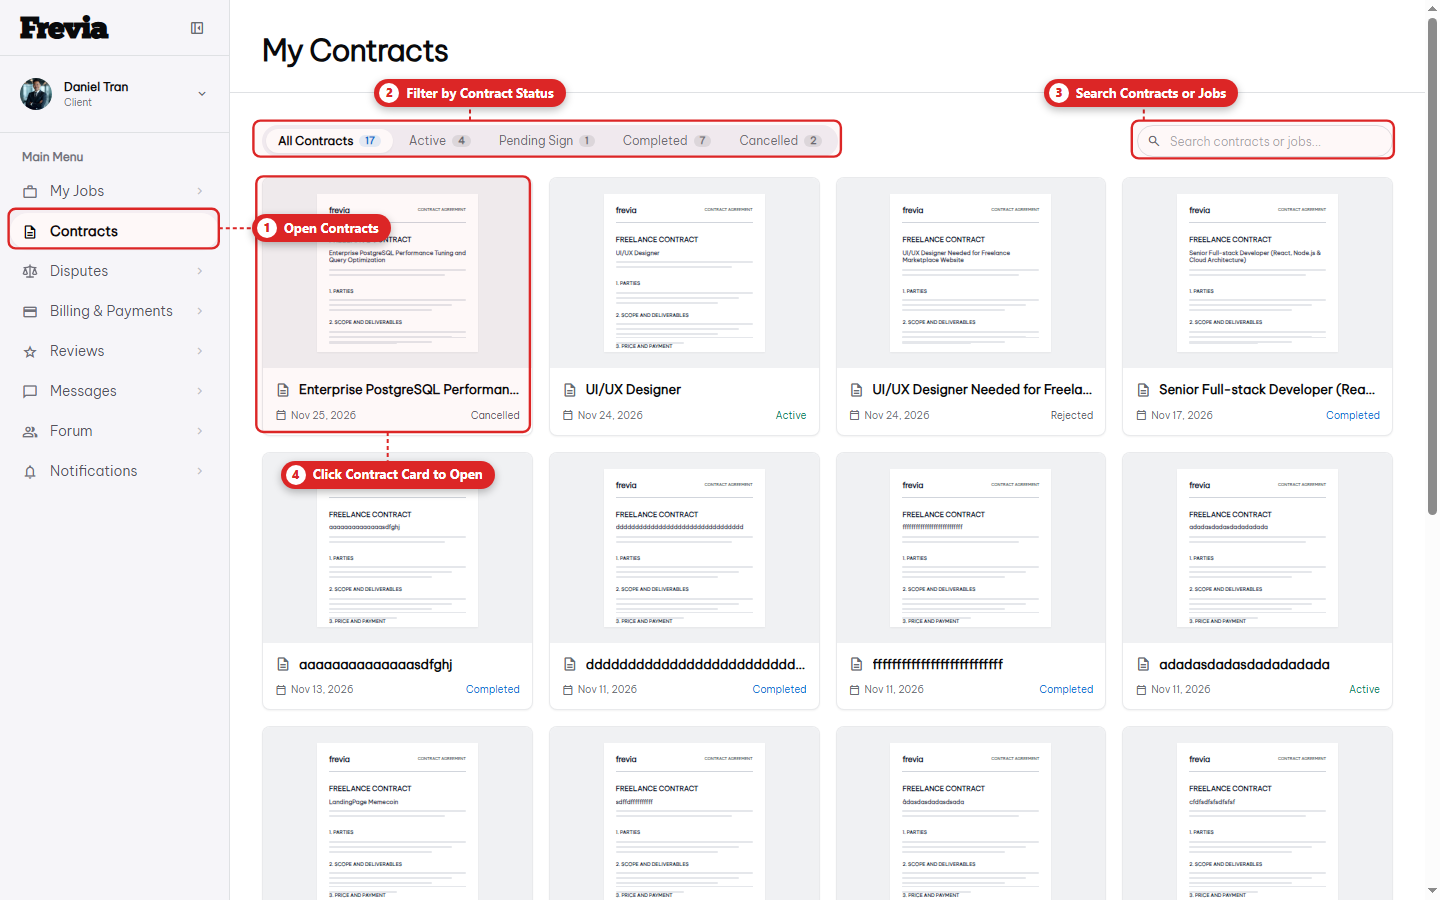
\includegraphics[width=0.90\textwidth]{images/contracts/m13_03_view_contracts_list_guide.png}
  \caption{My Contracts directory with status tabs, search, and document cards}
  \label{fig:m13_03_view_contracts_list}
\end{figure}
\Needspace{6\baselineskip}\paragraph{Step-by-Step User Guide:}
\begin{enumerate}[leftmargin=1.8em,itemsep=3pt]
  \item \rbadge{1} \textbf{Open Contracts:} Select \textbf{Contracts} in the left navigation sidebar.
  \item \rbadge{2} \textbf{Filter by Contract Status:} Switch across status tabs (\textbf{All Contracts}, \textbf{Active}, \textbf{Pending Sign}, \textbf{Completed}, \textbf{Cancelled}) with live badge counters.
  \item \rbadge{3} \textbf{Search Contracts or Jobs:} Type a job title or contract slug in \textit{Search contracts or jobs...} to narrow results.
  \item \rbadge{4} \textbf{Click Contract Card to Open:} Click any paper contract preview card to open its full agreement workspace.
\end{enumerate}
\Needspace{6\baselineskip}\paragraph{After You Submit (Result \& Troubleshooting):}
\begin{itemize}[leftmargin=1.5em,itemsep=2pt]
  \item \textbf{What Happens Next:} Paginated contracts associated with your account render chronologically with live lifecycle badges.
  \item \textbf{Troubleshooting \& Common Messages:} If no contracts match a status tab or keyword, a contextual empty state with clear-filters action appears.
\end{itemize}

% -----------------------------------------------------------------------------
\newpage
\subsubsection{M13.04 -- View Contract Details (UC-13.05)}

\begin{itemize}[leftmargin=1.5em,itemsep=2pt]
  \item \textbf{Screen Name \& Route Path:} Contract Detail Workspace -- \texttt{/[role]/\allowbreak{}contracts/\allowbreak{}[slug]}.
  \item \textbf{Target Actor:} Client, Freelancer.
  \item \Needspace{6\baselineskip}\textbf{Before You Begin:} You are a direct counterparty on the selected contract.
\end{itemize}
\begin{figure}[H]\centering
  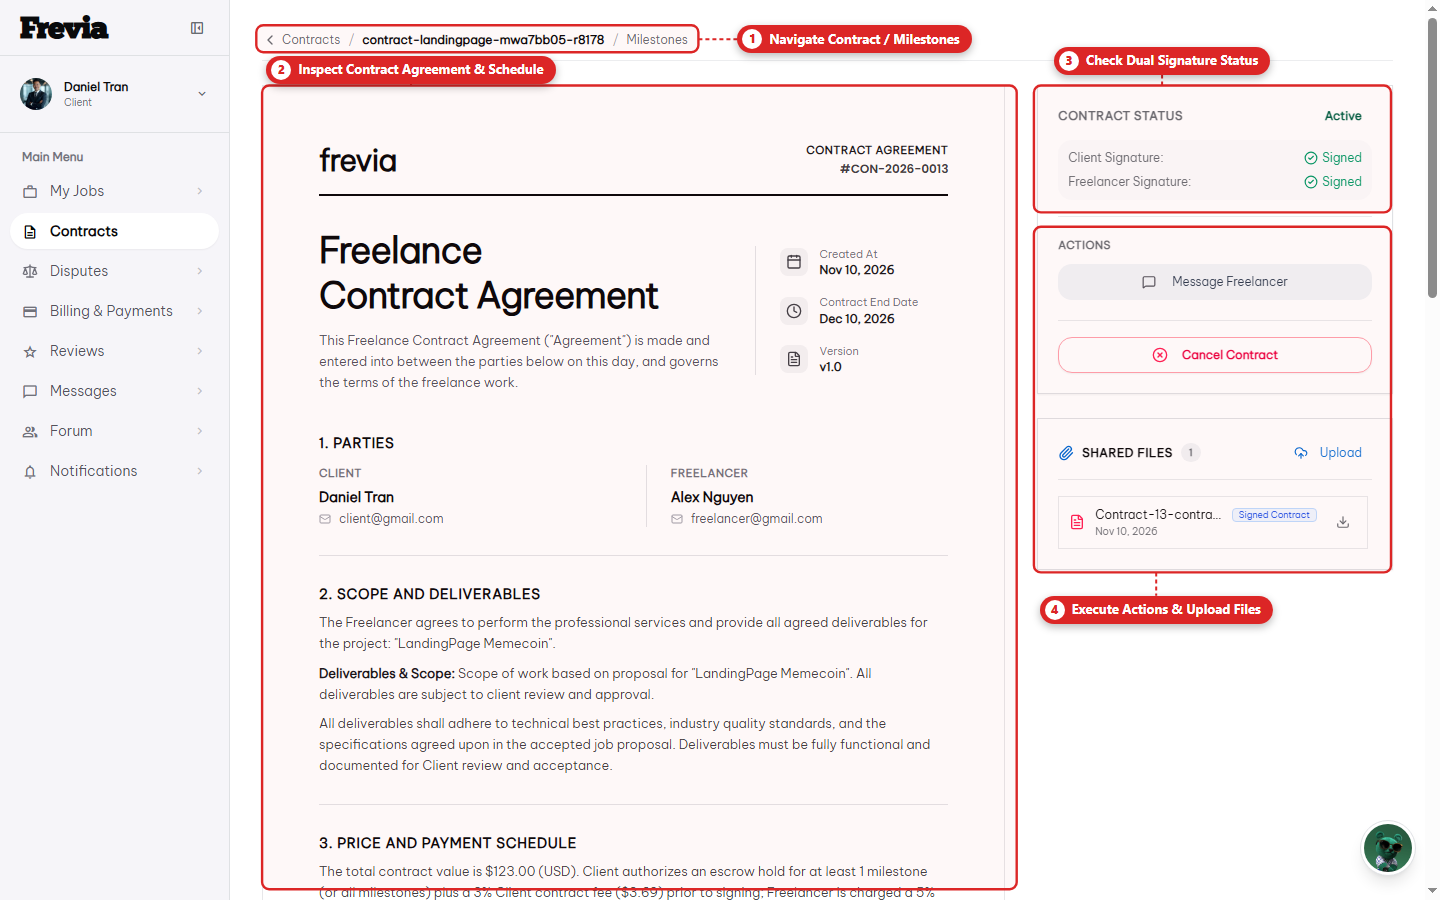
\includegraphics[width=0.90\textwidth]{images/contracts/m13_04_view_contract_detail_guide.png}
  \caption{Contract detail workspace displaying legal agreement, signatures, actions, and shared files}
  \label{fig:m13_04_view_contract_detail}
\end{figure}
\Needspace{6\baselineskip}\paragraph{Step-by-Step User Guide:}
\begin{enumerate}[leftmargin=1.8em,itemsep=3pt]
  \item \rbadge{1} \textbf{Navigate Contract / Milestones:} Use the top breadcrumb to switch between \textbf{Contracts}, the current agreement, and the \textbf{Milestones} workspace.
  \item \rbadge{2} \textbf{Inspect Contract Agreement \& Schedule:} Review Sections 1--3 covering Parties, Scope \& Deliverables, and Price \& Payment Schedule.
  \item \rbadge{3} \textbf{Check Dual Signature Status:} Monitor Client and Freelancer signature states in the \textbf{CONTRACT STATUS} panel.
  \item \rbadge{4} \textbf{Execute Actions \& Upload Files:} Use \textbf{ACTIONS} (\textit{Message Freelancer/Client}, \textit{Cancel Contract}, or \textit{Complete Contract}) and manage \textbf{SHARED FILES}.
\end{enumerate}
\Needspace{6\baselineskip}\paragraph{After You Submit (Result \& Troubleshooting):}
\begin{itemize}[leftmargin=1.5em,itemsep=2pt]
  \item \textbf{What Happens Next:} Full agreement state, signature timestamps, actions, and shared attachments render in real time.
  \item \textbf{Troubleshooting \& Common Messages:} Attempting to open a contract belonging to other users returns HTTP 403 Forbidden.
\end{itemize}

% -----------------------------------------------------------------------------
\newpage
\subsubsection{M13.05 -- Sign Contract Agreement (UC-13.06)}

\begin{itemize}[leftmargin=1.5em,itemsep=2pt]
  \item \textbf{Screen Name \& Route Path:} Sign Contract Modal -- \texttt{/[role]/\allowbreak{}contracts/\allowbreak{}[slug]}.
  \item \textbf{Target Actor:} Client, Freelancer.
  \item \Needspace{6\baselineskip}\textbf{Before You Begin:} Contract hold deposit has been authorized (\texttt{PENDING\_SIGN}) and the Client signs before the Freelancer countersigns.
\end{itemize}
\begin{figure}[H]\centering
  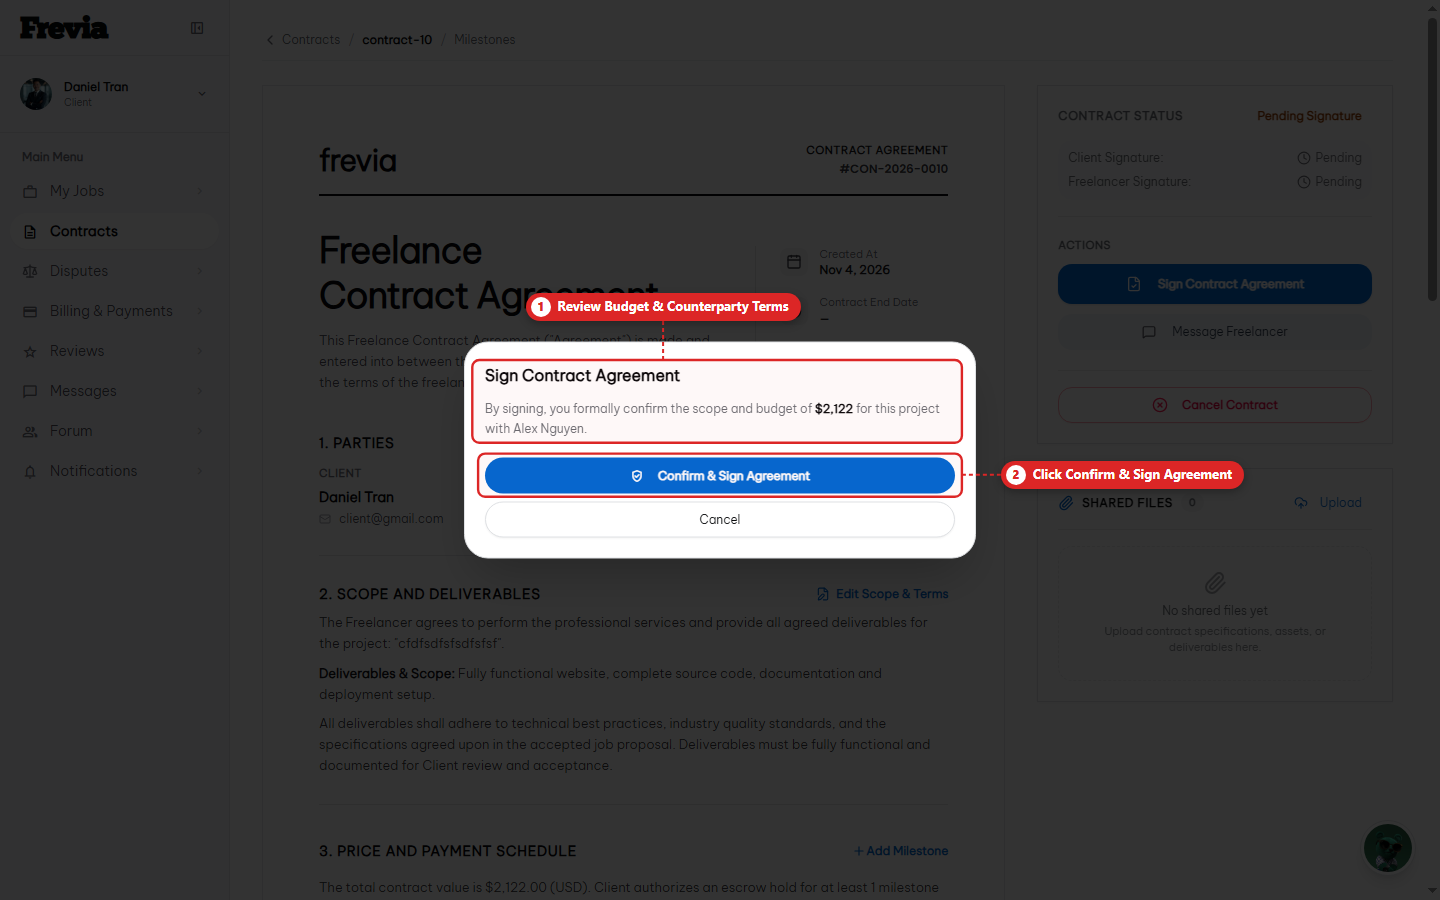
\includegraphics[width=0.90\textwidth]{images/contracts/m13_05_sign_contract_guide.png}
  \caption{Sign Contract Agreement confirmation modal}
  \label{fig:m13_05_sign_contract}
\end{figure}
\Needspace{6\baselineskip}\paragraph{Step-by-Step User Guide:}
\begin{enumerate}[leftmargin=1.8em,itemsep=3pt]
  \item \rbadge{1} \textbf{Review Budget \& Counterparty Terms:} Click \textbf{Sign Contract Agreement} in the Actions sidebar, then verify the committed contract amount and counterparty in the modal.
  \item \rbadge{2} \textbf{Click Confirm \& Sign Agreement:} Click the blue \textbf{Confirm \& Sign Agreement} button to record your legally binding timestamped signature.
\end{enumerate}
\Needspace{6\baselineskip}\paragraph{After You Submit (Result \& Troubleshooting):}
\begin{itemize}[leftmargin=1.5em,itemsep=2pt]
  \item \textbf{What Happens Next:} Once both Client and Freelancer sign, the contract transitions to \texttt{ACTIVE}, captures the authorized first milestone + 3\% fee hold via Stripe, and generates the signed PDF copy.
  \item \textbf{Troubleshooting \& Common Messages:} Freelancers see \textit{``Waiting for the Client to sign first before you can countersign''} until the Client's signature is recorded.
\end{itemize}

% -----------------------------------------------------------------------------
\newpage
\subsubsection{M13.06 -- Export Signed Contract PDF (UC-13.07)}

\begin{itemize}[leftmargin=1.5em,itemsep=2pt]
  \item \textbf{Screen Name \& Route Path:} Contract Detail / Shared Files -- \texttt{/[role]/\allowbreak{}contracts/\allowbreak{}[slug]}.
  \item \textbf{Target Actor:} Client, Freelancer.
  \item \Needspace{6\baselineskip}\textbf{Before You Begin:} The contract agreement is active or completed with a generated PDF document (\texttt{GET /api/contracts/:id/pdf}).
\end{itemize}
\begin{figure}[H]\centering
  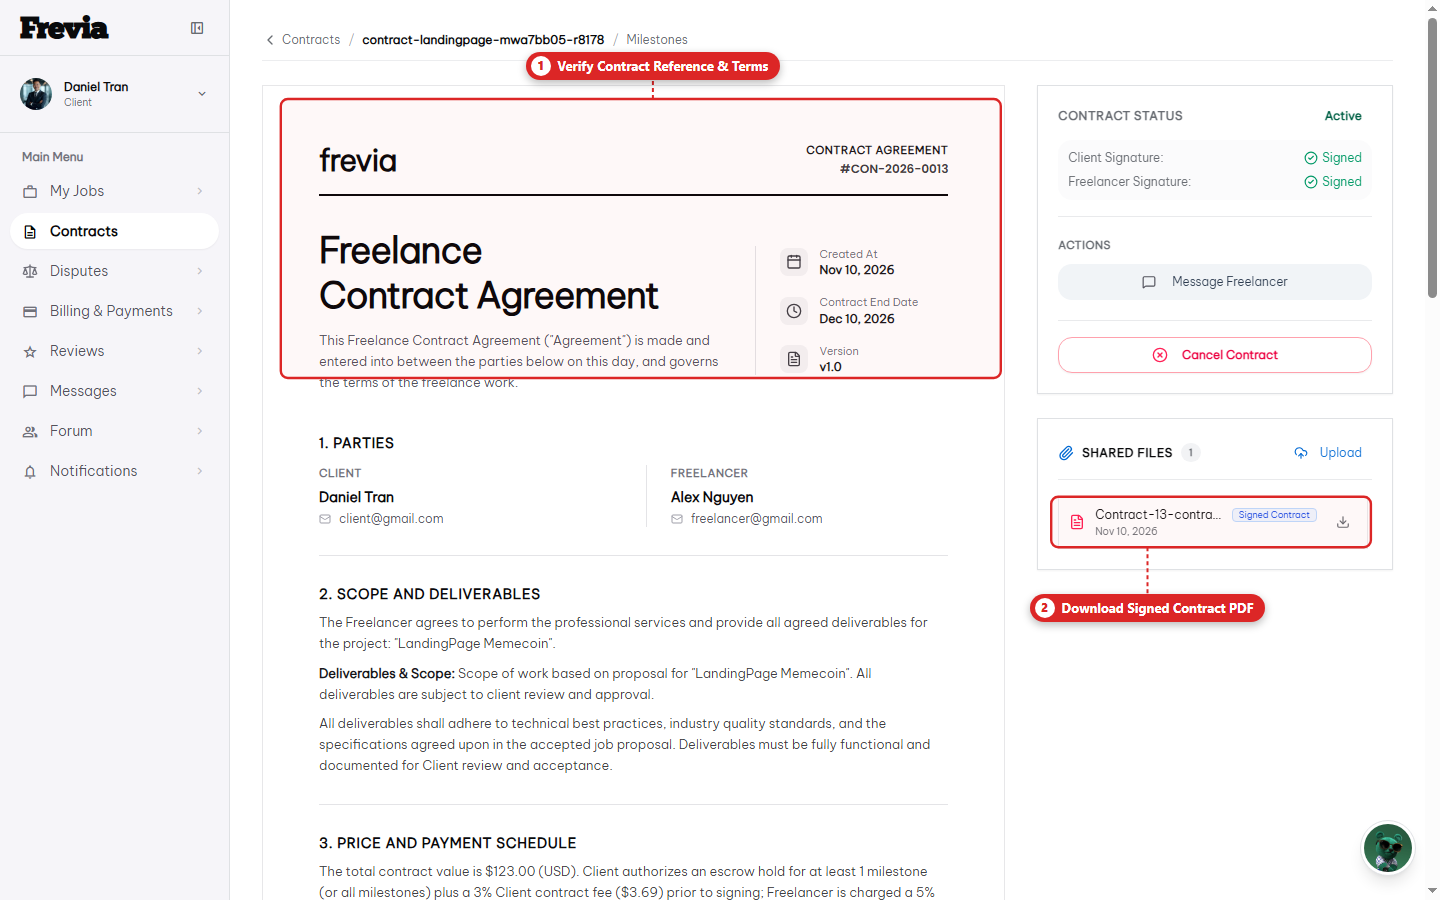
\includegraphics[width=0.90\textwidth]{images/contracts/m13_06_export_contract_pdf_guide.png}
  \caption{Downloading the generated signed Contract PDF agreement}
  \label{fig:m13_06_export_contract_pdf}
\end{figure}
\Needspace{6\baselineskip}\paragraph{Step-by-Step User Guide:}
\begin{enumerate}[leftmargin=1.8em,itemsep=3pt]
  \item \rbadge{1} \textbf{Verify Contract Reference \& Terms:} Confirm the Contract ID (e.g., \texttt{\#CON-2026-0013}), effective dates, and version on the paper agreement.
  \item \rbadge{2} \textbf{Download Signed Contract PDF:} In the right-hand \textbf{SHARED FILES} panel (or contract card actions menu), click the download icon next to the \textbf{Signed Contract} PDF entry.
\end{enumerate}
\Needspace{6\baselineskip}\paragraph{After You Submit (Result \& Troubleshooting):}
\begin{itemize}[leftmargin=1.5em,itemsep=2pt]
  \item \textbf{What Happens Next:} The browser downloads a formatted A4 PDF containing full party details, deliverables, payment schedule, and signature metadata.
  \item \textbf{Troubleshooting \& Common Messages:} Non-participants are blocked from streaming or exporting another party's contract PDF.
\end{itemize}

% -----------------------------------------------------------------------------
\newpage
\subsubsection{M13.07 -- Cancel Contract (UC-13.08)}

\begin{itemize}[leftmargin=1.5em,itemsep=2pt]
  \item \textbf{Screen Name \& Route Path:} Cancel Contract Confirmation Modal -- \texttt{/[role]/\allowbreak{}contracts/\allowbreak{}[slug]}.
  \item \textbf{Target Actor:} Client, Freelancer.
  \item \Needspace{6\baselineskip}\textbf{Before You Begin:} Click \textbf{Cancel Contract} in the Actions sidebar of an eligible contract.
\end{itemize}
\begin{figure}[H]\centering
  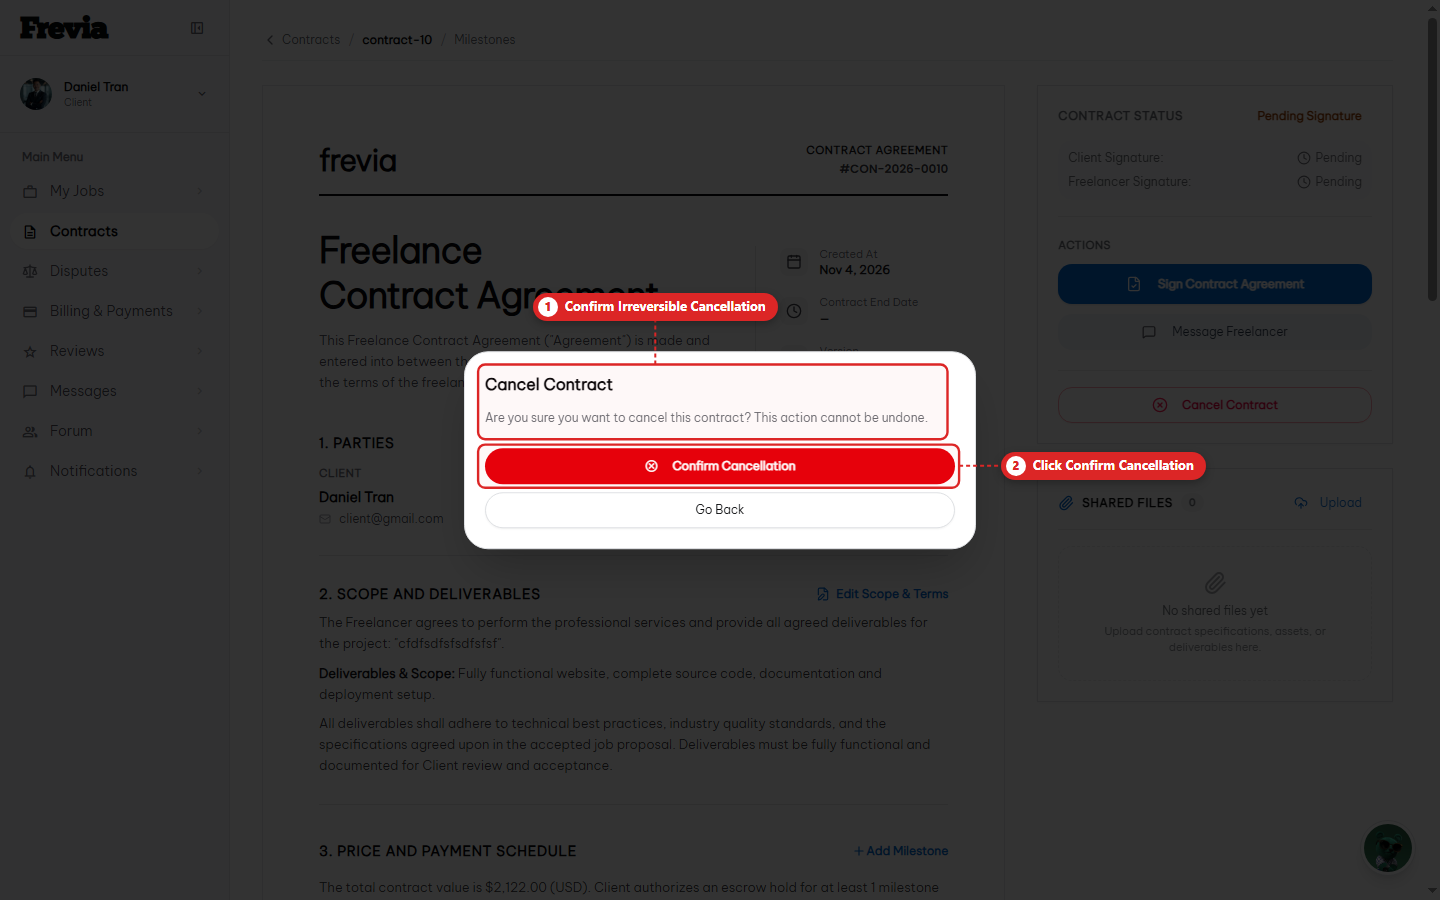
\includegraphics[width=0.90\textwidth]{images/contracts/m13_07_cancel_contract_guide.png}
  \caption{Cancel Contract confirmation dialog}
  \label{fig:m13_07_cancel_contract}
\end{figure}
\Needspace{6\baselineskip}\paragraph{Step-by-Step User Guide:}
\begin{enumerate}[leftmargin=1.8em,itemsep=3pt]
  \item \rbadge{1} \textbf{Confirm Irreversible Cancellation:} Review the warning noting that contract cancellation cannot be undone (or click \textbf{Go Back} to abort).
  \item \rbadge{2} \textbf{Click Confirm Cancellation:} Click the red \textbf{Confirm Cancellation} button to cancel the agreement.
\end{enumerate}
\Needspace{6\baselineskip}\paragraph{After You Submit (Result \& Troubleshooting):}
\begin{itemize}[leftmargin=1.5em,itemsep=2pt]
  \item \textbf{What Happens Next:} Contract status changes to \texttt{CANCELLED}; uncaptured Stripe card holds are automatically released and job positions reopen if applicable.
  \item \textbf{Troubleshooting \& Common Messages:} Active contracts with disputed or already-released funded milestones require the Resolution Center rather than direct cancellation.
\end{itemize}

% -----------------------------------------------------------------------------
\newpage
\subsubsection{M13.08 -- Complete Contract (UC-13.03)}

\begin{itemize}[leftmargin=1.5em,itemsep=2pt]
  \item \textbf{Screen Name \& Route Path:} Complete Contract Modal -- \texttt{/client/\allowbreak{}contracts/\allowbreak{}[slug]}.
  \item \textbf{Target Actor:} Client.
  \item \Needspace{6\baselineskip}\textbf{Before You Begin:} Contract is \texttt{ACTIVE} and all agreed milestones have been reviewed, approved, and released.
\end{itemize}
\begin{figure}[H]\centering
  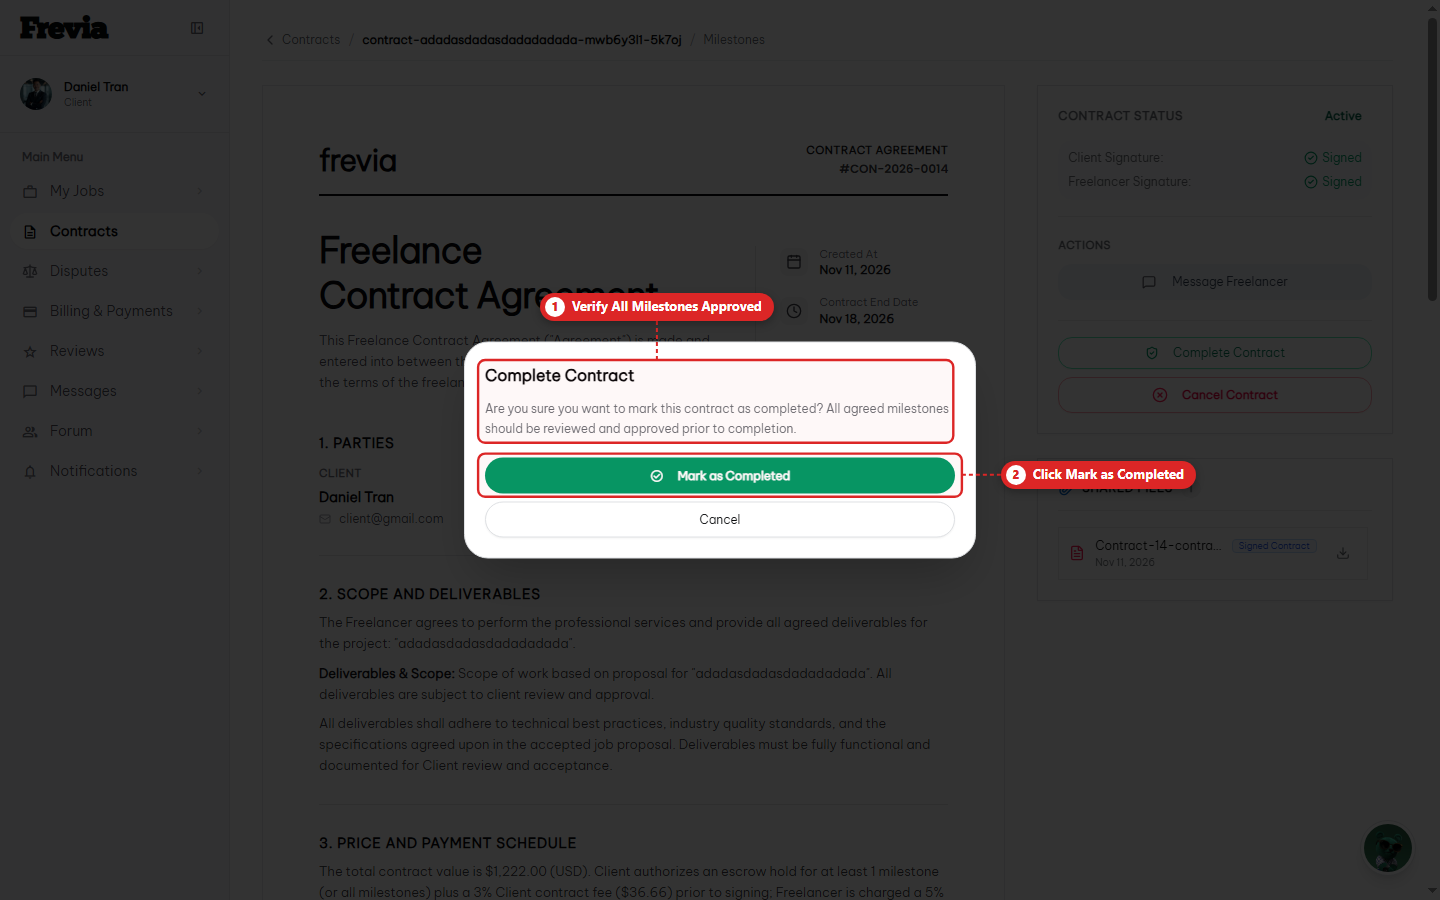
\includegraphics[width=0.90\textwidth]{images/contracts/m13_08_complete_contract_guide.png}
  \caption{Complete Contract confirmation dialog for finalizing an active engagement}
  \label{fig:m13_08_complete_contract}
\end{figure}
\Needspace{6\baselineskip}\paragraph{Step-by-Step User Guide:}
\begin{enumerate}[leftmargin=1.8em,itemsep=3pt]
  \item \rbadge{1} \textbf{Verify All Milestones Approved:} Click \textbf{Complete Contract} in the Actions sidebar and confirm the prerequisite check stating all milestones must be approved prior to completion.
  \item \rbadge{2} \textbf{Click Mark as Completed:} Click the green \textbf{Mark as Completed} button to finalize the engagement.
\end{enumerate}
\Needspace{6\baselineskip}\paragraph{After You Submit (Result \& Troubleshooting):}
\begin{itemize}[leftmargin=1.5em,itemsep=2pt]
  \item \textbf{What Happens Next:} The contract status transitions to \texttt{COMPLETED}, unlocking mutual Client--Freelancer reviews in the Reviews workspace.
  \item \textbf{Troubleshooting \& Common Messages:} If any milestone remains pending, funded-unreleased, or disputed, the backend rejects completion with HTTP 422.
\end{itemize}

% -----------------------------------------------------------------------------
\newpage
\subsubsection{M13.09 -- View Contract Shared Files (UC-13.09)}

\begin{itemize}[leftmargin=1.5em,itemsep=2pt]
  \item \textbf{Screen Name \& Route Path:} Contract Detail Sidebar -- \texttt{/[role]/\allowbreak{}contracts/\allowbreak{}[slug]}.
  \item \textbf{Target Actor:} Client, Freelancer.
  \item \Needspace{6\baselineskip}\textbf{Before You Begin:} Contract workspace is open and at least one file or signed PDF has been attached.
\end{itemize}
\begin{figure}[H]\centering
  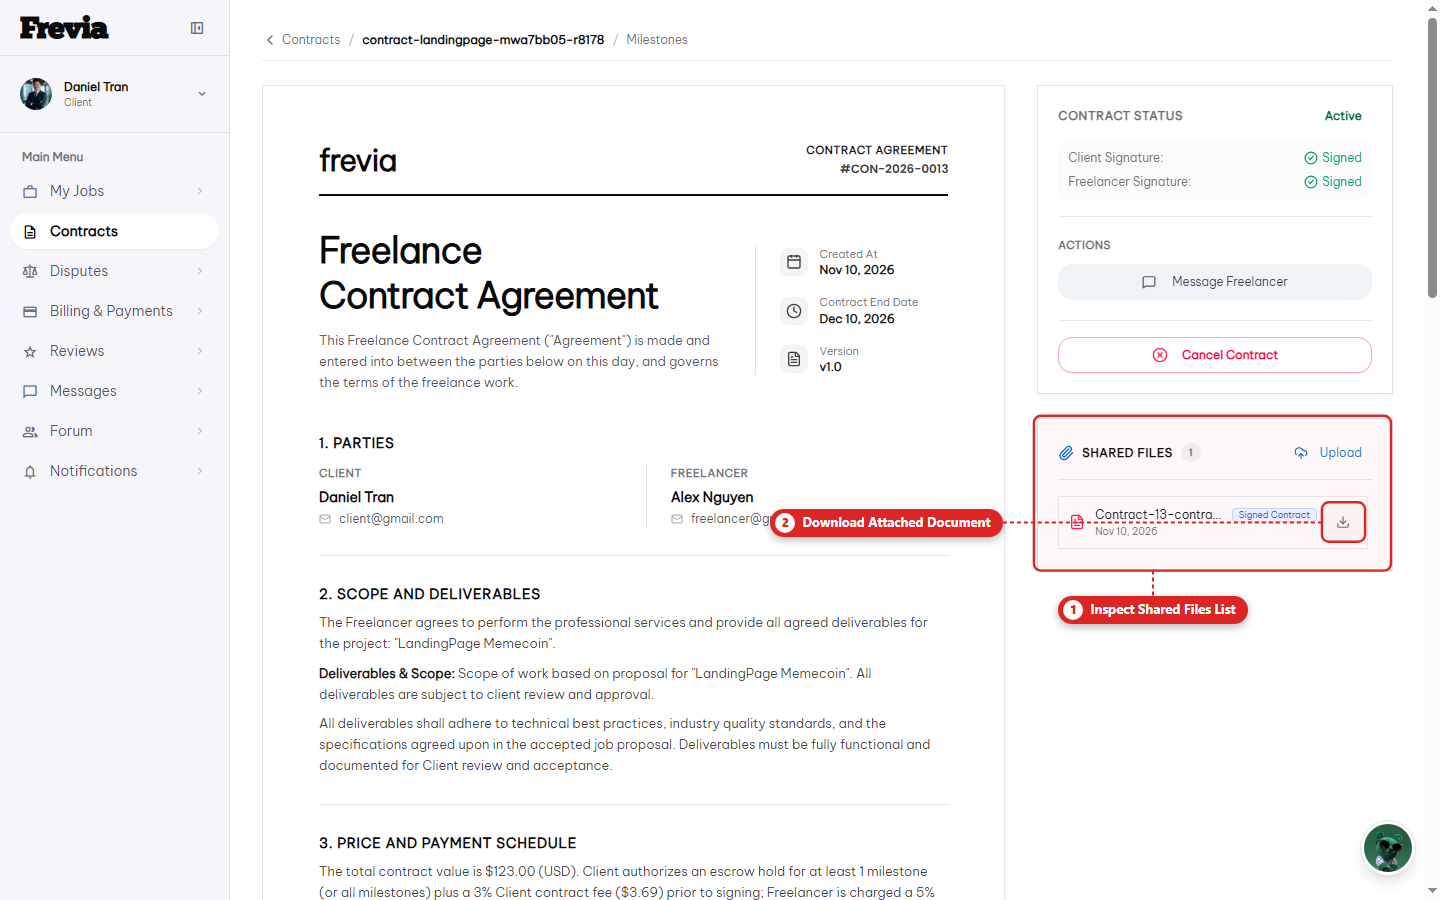
\includegraphics[width=0.90\textwidth]{images/contracts/m13_09_view_contract_files_guide.png}
  \caption{Shared Files panel listing contract documents and download triggers}
  \label{fig:m13_09_view_contract_files}
\end{figure}
\Needspace{6\baselineskip}\paragraph{Step-by-Step User Guide:}
\begin{enumerate}[leftmargin=1.8em,itemsep=3pt]
  \item \rbadge{1} \textbf{Inspect Shared Files List:} Locate the \textbf{SHARED FILES} card in the bottom-right sidebar displaying filename, upload timestamp, and tag badges.
  \item \rbadge{2} \textbf{Download Attached Document:} Click the download icon on any file row to retrieve the document directly to your device.
\end{enumerate}
\Needspace{6\baselineskip}\paragraph{After You Submit (Result \& Troubleshooting):}
\begin{itemize}[leftmargin=1.5em,itemsep=2pt]
  \item \textbf{What Happens Next:} Authorized counterparties download contract attachments cleanly over Cloudinary or protected stream endpoints.
  \item \textbf{Troubleshooting \& Common Messages:} Empty contracts display a placeholder prompt inviting parties to upload specifications or assets.
\end{itemize}

% -----------------------------------------------------------------------------
\newpage
\subsubsection{M13.10 -- Upload Contract File (UC-13.10)}

\begin{itemize}[leftmargin=1.5em,itemsep=2pt]
  \item \textbf{Screen Name \& Route Path:} Contract Detail Workspace -- \texttt{/[role]/\allowbreak{}contracts/\allowbreak{}[slug]}.
  \item \textbf{Target Actor:} Client, Freelancer.
  \item \Needspace{6\baselineskip}\textbf{Before You Begin:} You have read/write access to the contract and a valid specification document, archive, or image ready locally.
\end{itemize}
\begin{figure}[H]\centering
  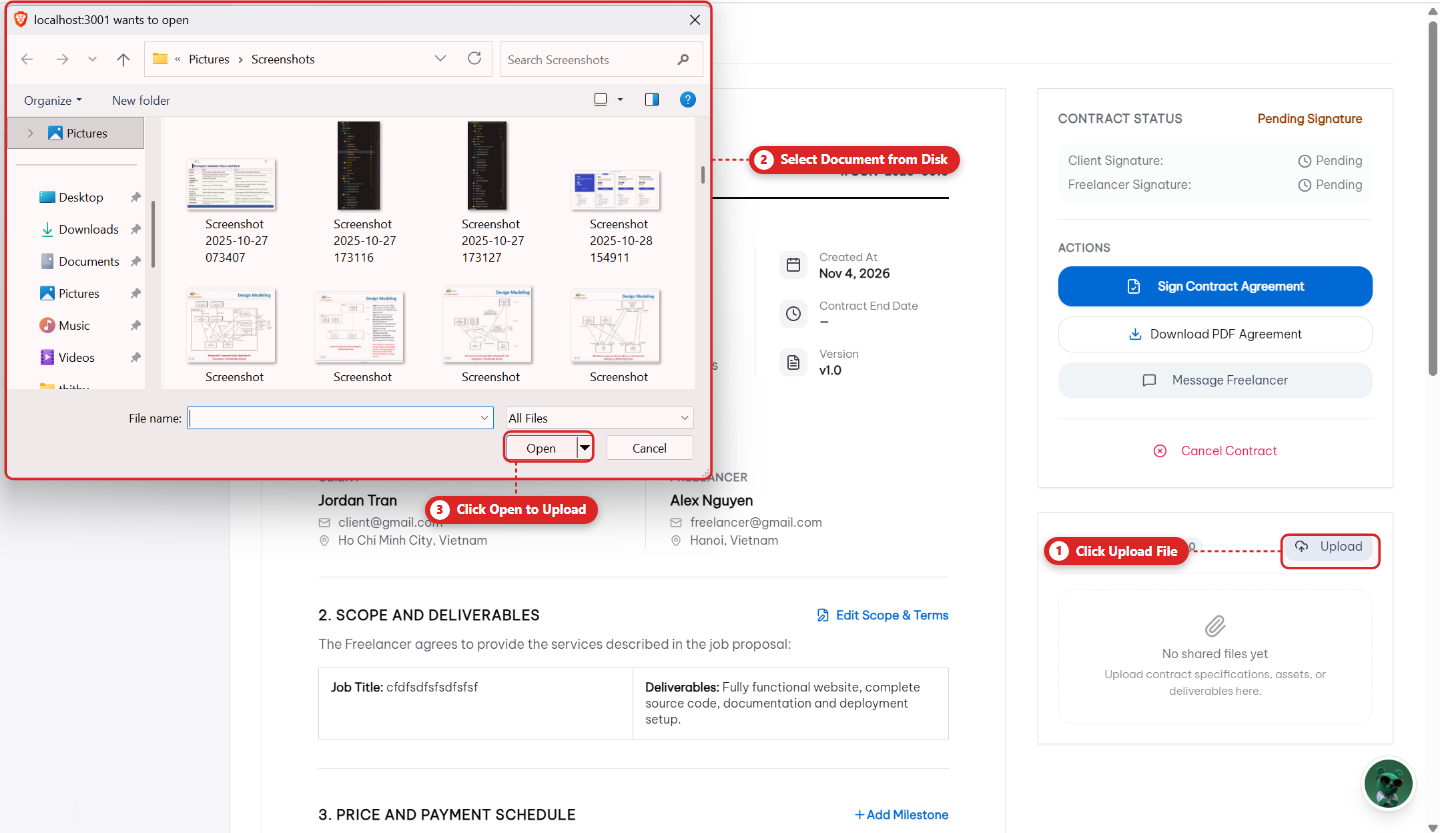
\includegraphics[width=0.90\textwidth]{images/contracts/m13_10_upload_contract_file_guide.png}
  \caption{Uploading a shared file attachment via the contract workspace}
  \label{fig:m13_10_upload_contract_file}
\end{figure}
\Needspace{6\baselineskip}\paragraph{Step-by-Step User Guide:}
\begin{enumerate}[leftmargin=1.8em,itemsep=3pt]
  \item \rbadge{1} \textbf{Click Upload File:} Click \textbf{Upload} at the top-right corner of the \textbf{SHARED FILES} card.
  \item \rbadge{2} \textbf{Select Document from Disk:} Browse local folders in the operating system file chooser and select the specification, asset, or brief file.
  \item \rbadge{3} \textbf{Click Open to Upload:} Click \textbf{Open} to send the multipart payload to the API and link it to the contract.
\end{enumerate}
\Needspace{6\baselineskip}\paragraph{After You Submit (Result \& Troubleshooting):}
\begin{itemize}[leftmargin=1.5em,itemsep=2pt]
  \item \textbf{What Happens Next:} The uploaded file immediately appears in \textbf{SHARED FILES} for both Client and Freelancer.
  \item \textbf{Troubleshooting \& Common Messages:} Oversized files or unsupported MIME formats display an upload validation toast; cancelled/completed read-only contracts block new uploads.
\end{itemize}

% -----------------------------------------------------------------------------
\newpage
\subsubsection{M13.11 -- Delete Contract File (UC-13.11)}

\begin{itemize}[leftmargin=1.5em,itemsep=2pt]
  \item \textbf{Screen Name \& Route Path:} Delete Shared File Modal -- \texttt{/[role]/\allowbreak{}contracts/\allowbreak{}[slug]}.
  \item \textbf{Target Actor:} Client (or original file uploader).
  \item \Needspace{6\baselineskip}\textbf{Before You Begin:} Click the trash icon beside a deletable entry in \textbf{SHARED FILES}.
\end{itemize}
\begin{figure}[H]\centering
  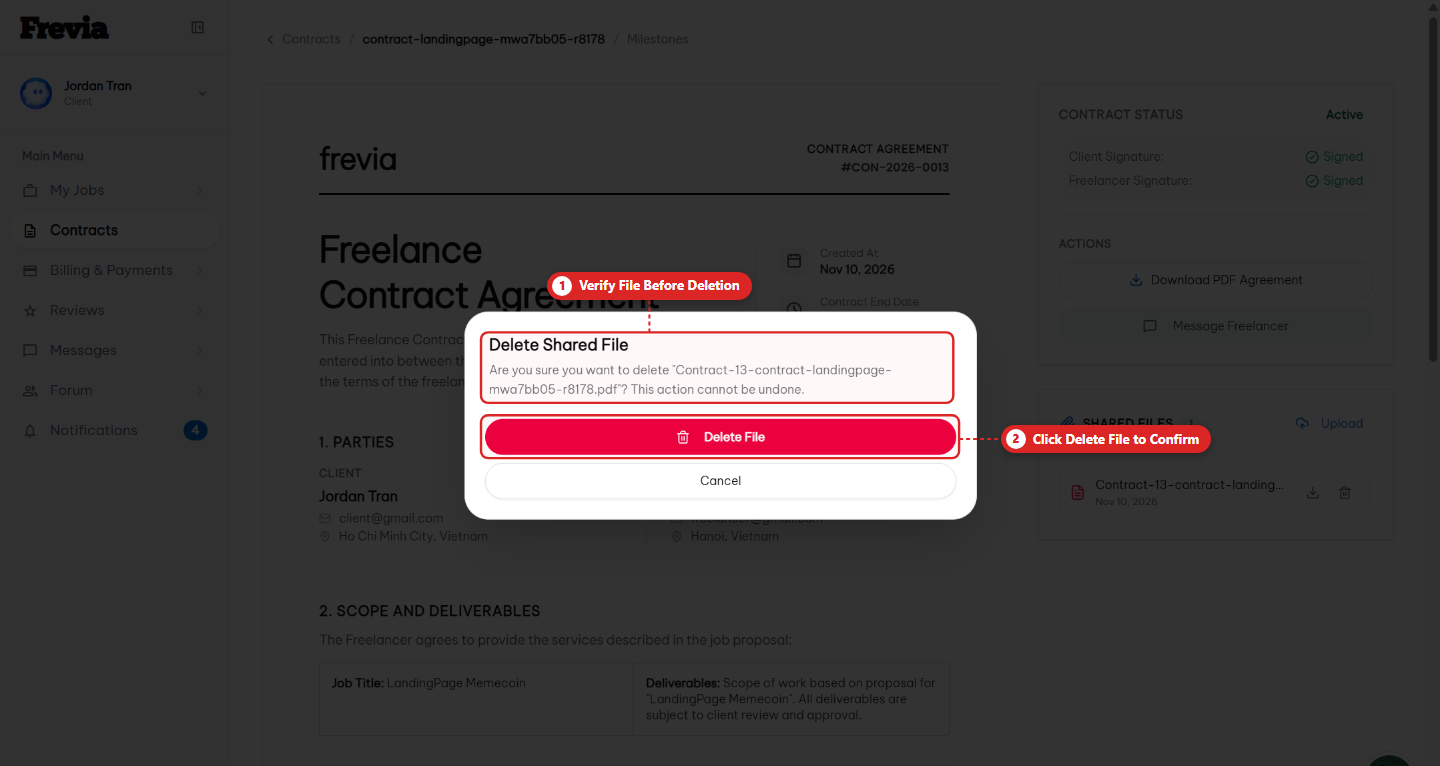
\includegraphics[width=0.90\textwidth]{images/contracts/m13_11_delete_contract_file_guide.png}
  \caption{Delete Shared File confirmation dialog}
  \label{fig:m13_11_delete_contract_file}
\end{figure}
\Needspace{6\baselineskip}\paragraph{Step-by-Step User Guide:}
\begin{enumerate}[leftmargin=1.8em,itemsep=3pt]
  \item \rbadge{1} \textbf{Verify File Before Deletion:} Check the filename shown in the confirmation prompt (\textit{``Are you sure you want to delete...''}).
  \item \rbadge{2} \textbf{Click Delete File to Confirm:} Click the red \textbf{Delete File} button (or \textbf{Cancel} to preserve the attachment).
\end{enumerate}
\Needspace{6\baselineskip}\paragraph{After You Submit (Result \& Troubleshooting):}
\begin{itemize}[leftmargin=1.5em,itemsep=2pt]
  \item \textbf{What Happens Next:} The shared file record is removed and the counterparty's file count badge decrements immediately.
  \item \textbf{Troubleshooting \& Common Messages:} Unauthorized users attempting to delete files uploaded by the other party receive HTTP 403 Forbidden.
\end{itemize}

% -----------------------------------------------------------------------------
\newpage
\subsubsection{M13.12 -- Reject Contract Offer (UC-13.12)}

\begin{itemize}[leftmargin=1.5em,itemsep=2pt]
  \item \textbf{Screen Name \& Route Path:} Decline Contract Offer Modal -- \texttt{/freelancer/\allowbreak{}contracts/\allowbreak{}[slug]}.
  \item \textbf{Target Actor:} Freelancer.
  \item \Needspace{6\baselineskip}\textbf{Before You Begin:} Contract is awaiting Freelancer acceptance/signature (\texttt{PENDING\_SIGN} or \texttt{AWAITING\_PAYMENT}).
\end{itemize}
\begin{figure}[H]\centering
  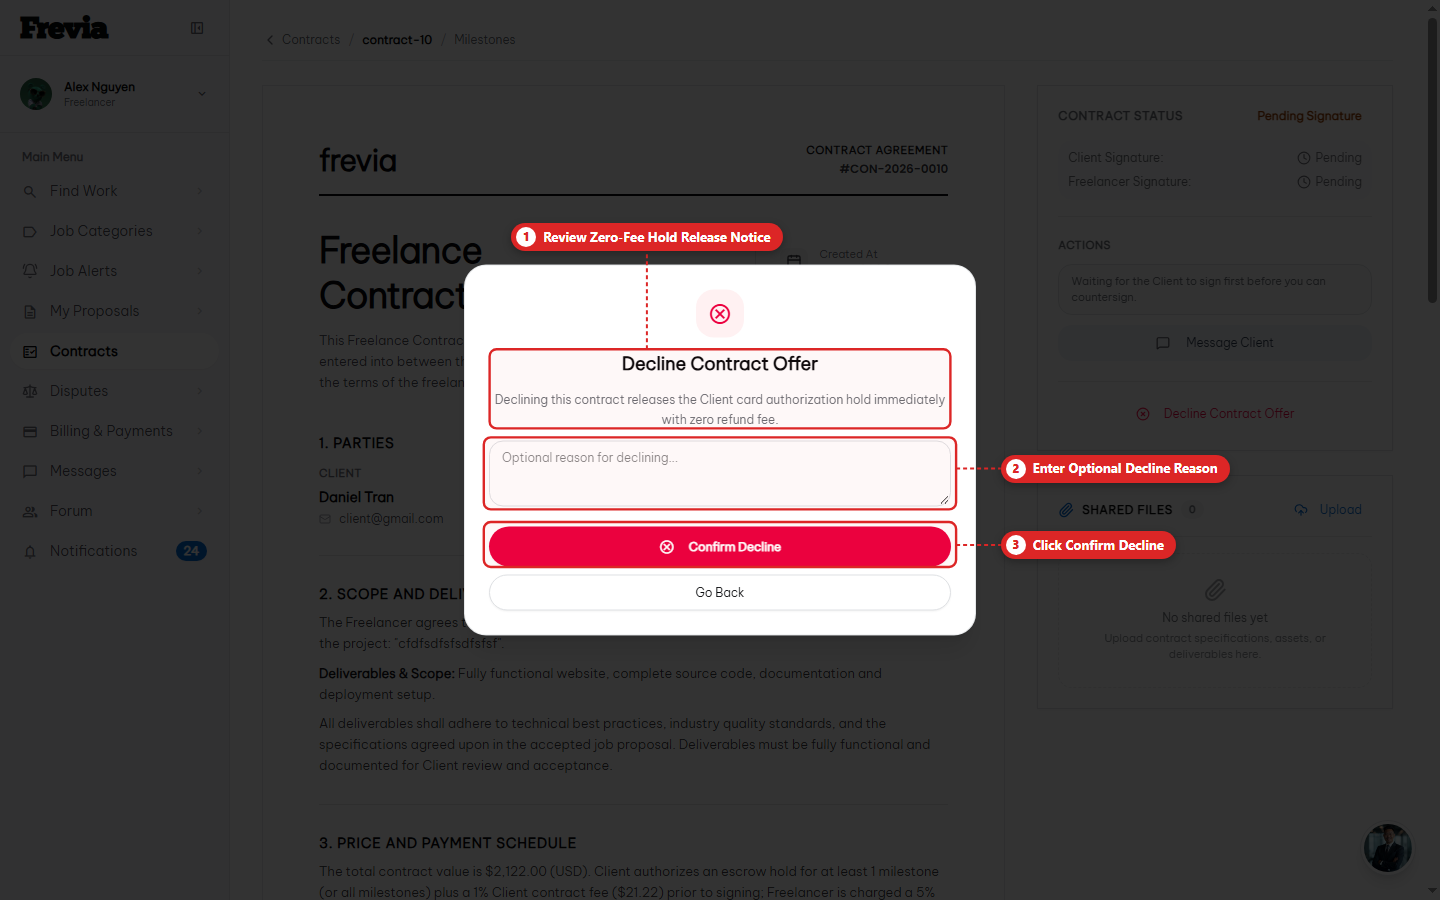
\includegraphics[width=0.90\textwidth]{images/contracts/m13_12_reject_contract_offer_guide.png}
  \caption{Decline Contract Offer dialog explaining automatic Stripe hold release}
  \label{fig:m13_12_reject_contract_offer}
\end{figure}
\Needspace{6\baselineskip}\paragraph{Step-by-Step User Guide:}
\begin{enumerate}[leftmargin=1.8em,itemsep=3pt]
  \item \rbadge{1} \textbf{Review Zero-Fee Hold Release Notice:} Click \textbf{Decline Contract Offer} in Actions and confirm the notice stating the Client's card hold will be released immediately with zero refund fee.
  \item \rbadge{2} \textbf{Enter Optional Decline Reason:} Type why you are declining (e.g., timeline conflict or revised scope request) in the textarea.
  \item \rbadge{3} \textbf{Click Confirm Decline:} Click the red \textbf{Confirm Decline} button to decline the contract offer.
\end{enumerate}
\Needspace{6\baselineskip}\paragraph{After You Submit (Result \& Troubleshooting):}
\begin{itemize}[leftmargin=1.5em,itemsep=2pt]
  \item \textbf{What Happens Next:} Contract status becomes \texttt{REJECTED}, any authorized hold PaymentIntent is canceled in Stripe, and the Client is notified.
  \item \textbf{Troubleshooting \& Common Messages:} Contracts already signed by both sides (\texttt{ACTIVE}) cannot be declined via this modal and require cancellation or dispute workflows.
\end{itemize}
